\section{Introduction to Prefix search}
The indexes created so far only return the list of article titles where there is an exact match of the query. This can inhibit the user experience as this search form might miss relevant articles where a buzzword simply is written in another tense or in  pluralism, which could add different suffixes to the word. To improve the user experience of the search engine and to explore the data structure of tries indexes that support prefix search where implemented.

Prefix search enables users to input partial words and retrieve relevant results that match the given prefix. If the user want to search for a prefix they simply need to add a star as a suffix of their query. For instance, when typing "pre*" in a search engine, it the indexes will return all articles titles of articles where a word with the prefix "pre" is present. 

To implement prefix search efficiently, one effective data structure that can be employed is a trie, also known as a prefix tree. A trie is a tree-like structure that stores a database, with each node representing a character in the string. Tries offer an optimized approach for prefix search by allowing rapid traversal and retrieval of words based on their prefixes.

Figure \ref{fig:trie-st-example} shows an example of a tire for the database "BE, BEE, BEEN, BAT, CAT, HAT". It is commonly used to add extra end notes containing a special sign such as "\$" to indicate that a word has ended in its parent note. Both prefix indexes do not use these extra notes. However, each note can have an article list, indicating that the word ending in this node, is present in the articles in the article list.  

\begin{figure}[ht!]
    \centering
    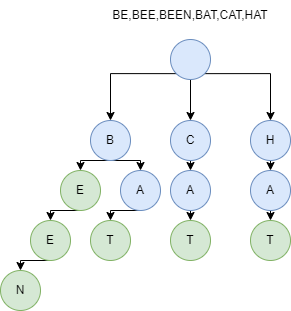
\includegraphics[width=.5\textwidth]{LaTeX/Figures/trie.png}
    \caption{Example of a trie for the database BE,BEE,BEEN,BAT,CAT,HAT. Green nodes are end notes meaning that the note also points to an article list.}
    \label{fig:trie-st-example}
\end{figure}